\documentclass[conference]{IEEEtran}
\IEEEoverridecommandlockouts
% The preceding line is only needed to identify funding in the first footnote. If that is unneeded, please comment it out.
\usepackage{cite}
\usepackage{amsmath,amssymb,amsfonts}
\usepackage{algorithmic}
\usepackage{graphicx}
\usepackage{textcomp}
\usepackage{xcolor}
\usepackage{multicol}
\def\BibTeX{{\rm B\kern-.05em{\sc i\kern-.025em b}\kern-.08em
   T\kern-.1667em\lower.7ex\hbox{E}\kern-.125emX}}
\begin{document}

\title{A theoretical analysis of the Keep Network random beacon using agent based modeling \\
\thanks{Identify applicable funding agency here. If none, delete this.}
}

\author{\IEEEauthorblockN{Prashanth Irudayaraj}
\IEEEauthorblockA{\textit{Keep Network} \\
prashanth@keep.network}

\and
\IEEEauthorblockN{Antonio Cordozo}
\IEEEauthorblockA{\textit{Keep Network} \\
antonio@keep.network}

\and
\IEEEauthorblockN{Promethea Raschke}
\IEEEauthorblockA{\textit{Keep Network} \\
promethea@keep.network}

\and
\IEEEauthorblockN{Markus Fix}
\IEEEauthorblockA{\textit{Keep Network} \\
markus@keep.network}
}

\maketitle

\begin{abstract}
    ABM is an effective tool for analysis of complex systems with long term 
    emergent behavior. In this study we apply ABM to analyse the long term 
    behavior of Keep’s random beacon. We look for the emergence of steady 
    state behavior, at which point we evaluate the sensitivity of specific 
    group and signature characteristics to various parameters. The results 
    of this study illustrates the effectiveness of ABM as an aid to the design 
    of novel distributed systems. 

\end{abstract}

\begin{IEEEkeywords}
Token Engineering, Agent Based Model, Distributed Systems
\end{IEEEkeywords}

\section{Introduction}

\section{Agent Based Modeling (ABM)}
ABM has traditionally been a tool to simulate complex dynamic systems 
such as the spread of pathogens \cite{Bauer2009}, social psychology 
\cite{Smith2007}, and financial markets \cite{Feng2012}. It is well suited
to systems that resist simple analytical solutions due to the interaction of 
complex individual agents with varying attributes. As a bottom up approach, ABM
has been gaining in popularity over tradtional methods such as Discrete Event
Simulation, and can provide more convincing theoretical analysis than approaches
such as general equilibrium analysis \cite{Wang2018}.

The nascent field of token engineering is currently establishing its own set 
of tools and processes. As such, ABM lends itself well to analyzing these systems
to support the design process and evaluate system state after launch. In many situations,
agent based modeling maybe the only method to evaluate a cryptoeconomic system as many are
opaque and do not generate significant visible data. Similar to the field of astronomy, an
agent based model could be used to replicate observable system behavior and then infer
causes. 

\section{Analysis of Token based systems}
Klages-Mundt et al.\cite{klages2019stability} use agent based models to simulate a decentralized stable coin
system and shows how deleveraging sprial attacks could occur. Their model is also able
to explain real complex stable coin movements. Further, the study is able
to show theoretically that regions of stability and instability exist for such decentralized
stable coin systems. 

While not agent based, Chitra et al. \cite{chitra2019agent} effectively use discrete event simuation to provide
quantitative estimates of how economic incentives affect security. They use a custom simulation
environment to simulate Kadena's Chainweb, and provide insights into how simulation can guide
and optimize protocol development in a variety of contexts.

Discuss levels of complexity, with citations. Why greater complexity may
not get you much more insight. (ask Shruti?)

\section{Overview of the Keep Random Beacon}
The Keep Network random beacon uses a threshold relay simuliar to the one proposed
by DFINITY and based on the BLS signature scheme \cite{} (NEED CITATION)

\subsection{Role of the model in the design process}
The initial architecture of the Keep beacon was designed by (need input from Antonio)
what purpose did the simulation serve?

\section{Key research questions}
\subsection{When could steady state behavior emerge?}
Emergence of steady state behavior occurs as a confluence of several factors and is difficult
to predict at the design stage. Specifically, process that take several blocks to complete 
such as DKG that often occur asynchronously can create large swings in values such as number of active
groups or percentage of compromised groups. 

\subsection{How could node failures and group sizes affect system behavior?}
Nodes may go offline or fail entireley. Since their participation in groups is critical to the 
success of the threshold relay, it is important to understand the impact of various levels
of failure on group characteristics. In particular, failures can result in disproportionate ownership
of groups which may cause a byzantine fault to occur. 

\subsection{How could different stake distributions affect system behavior?}
Stake distributions can also skew ownership of groups and can lead to a byzantine fault. A more
centralized distribution could once again lead to a greater ownership of groups by a few entities
thus creating conditions for the group to be compromised. 

\section{Model Creation}

\subsection{Key Terms}
\begin{itemize}
\item Node: A computational entity with memory and computational power sufficient to to run a 
keep client
    
\item Node Owner: may own 1 or more nodes and can allocate different levels of stake to each node
    owned
    
\item Stake: A bond that make a node eligible to participate in a group 
    
\item Group: A collection of nodes who have successfully completed DKG together
    
\item DKG (Distributed Key Generation): The processes of generating keys for each node enabling
    them to sign using Keep's version of Threshold ECDSA \cite{Gennaro2018}.
    
\item Signature: The process of securely generating a random number using Threshold ECDSA \cite{Gennaro2018}
    
\item Ownership Percent: The level of ownership a specific entity has in a group or signature
    
\item Lynchpin: A node who's ownership exceeds the maximum malicious threshold
\end{itemize}

\subsection{Model Structure}
We construct the model using the MESA ABM framework (cite). MESA consists of an agent class with
attributes and methods. We generate 3 types of agents Nodes, Groups, and Signatures. TABLE shows 
the specific differences in each of these.

ADD table for Agent types


Decide whether all parameters should be listed?


The simulation model consists of the model class which instantiates the various agents
and steps through the simulation. At each step the state of the model and each agent
is updated. The scheduler manages the sequence of state changes. For this model we use
a simulataneous activation scheduler, which first stages updates for each agent and then 
advances them simultaneously.  (NEED TO CHECK SCHEDULER SEQUENCE AGAIN)

Usually steps measure a change in time. Therefore for our simulation we assume
1 step = 1 block.

\subsection{Runs}
We perform two sets of experiments to answer our research questions. 
\begin{itemize}

\item Single run: Our single run of 1000 steps provide a first look at the 
performance of the sim, quickly. We also use this first experiment to evaluate
when steady state behavior could occur. We also perform some initial evaluations
of the impact of different stake distributions.

\item Multiple runs: The second experiment consists of multiple runs with varying 
parameters. For each change in parameter we perform 6 runs. By varying parameters 
in these runs we attempt to identify sensitivity. We measure this sensitivity after
the start of steady state behavior which we identify in the single run. 
    
\end{itemize}

\subsection{Assumptions}

\textit{Stochastic Assumptions}

To simplify the model we make stochastic assumptions for exogenous processes.

\begin{itemize}

\item Node Connection Delay: We apply a random uniform distribution to a user specified range (NEED JUSTIFICATION OR A JUSTIFIED SAMPLING)
\item Node Connection Failure: This is one of the parameters we intend to adjust to test for sensitivity. Therefore we
randomly pick a percentage of nodes to fail using a uniform distribution.
\item Node Death: We uniform randomly pick nodes to die at a user specified rate.
\item Signature Delay: A delay between when a signature is triggered and when it is executed. We use a poisson distribution. (NEED JUSTIFICATION or REFERENCE)
\item Node Owner Assignment: We use a normal distribution to assign owners to nodes. (NEED JUSTIFICATION)
\end{itemize}

\textit{Stake distribution} 

Since one of our research questions involves understanding the effects of centralization
on system behavior, we use three different token distribution models with 
varying degrees of decentraliation to evaluate this impact. 

\begin{itemize}
\item Linear Distribution: We assume a simple linear distribution as our most 
decentralized case. We take 50000 stakes and allocate them linearly to 100 nodes
as shown in Figure \ref{fig:linear_distribution}

\begin{figure}
    \includegraphics[width=\linewidth]{linear.png}
    \caption{Linear Stage Distribution}
    \label{fig:linear_distribution}
\end{figure}

\item Ethereum Distribution: In the spectrum of decentralization, we assume 
ETH to be moderateley decentralized. We therefore take the distribution of the 
top 30 percent account holders and apply it with some normalization in Figure \ref{fig:eth_distribution}.
(NEED TO JUSTIFY TOP 30 PERCENT)

\begin{figure}
    \includegraphics[width=\linewidth]{eth_distribution.png}
    \caption{Top 30 Percent Ethereum Distribution}
    \label{fig:eth_distribution}
\end{figure}

\item Assumed Stake Distribution: Should we disclose?
\end{itemize}


Assumptions
Model Assumptions
    
\section{Verification and Validation}
Where possible, we use analytical methods to verify aspects of the sim. In the absence of 
real world data, this is our best way to increase confidence in simulation results.

\subsection{Group Selection}
We model group selection using a hypergeometric distribution. For our purposes, we assume the n draws to 
be the equivalent of selecting a group of n members, with k members being malicious. We draw the sample from
a population of N virtual stakers, with K stakers being malicious. 

\begin{equation}
    Pr(X = k) = \frac{{K \choose k} {N-K\choose n-k}}{{N \choose n}}
\end{equation}

Show analytical results in comparison with simulation?

\subsection{Compromised Groups}
We use the survival function of the hypergeometric distribution to determine
the likelihood of a group of n members being compromised. To do this we evaluate
the function at the max malicious threshold. (in the sim we have a separate compromised threshold)

\subsection{Node Attrition, Failures, and Inactivity}
We model Node attrition and failures as Binomial, and Inactivity as a function of 
the two.

Describe mathematically....

\subsection{Lynchpinned Signatures}


\subsection{Failed Signatures}


\section{Results}
\subsection{Emergence of steady state behavior}
Using the single run experiment, we discover that system consistently appears to 
stabalizes to steady state usually around 400 blocks, and usually due to normalization of bootstrapping states. 
However, final steady state values for the percentage of total groups that are compromised
appears to vary significantly and is dependent on the degree of concentration in the 
stake distribution. 

\subsection{Convergence pressures}
The model primarily converges to steady state due to factors such as
signature request frequency, node availability, and group creation/expiration. We discuss a few
steady state values of interest.

\textit{Active group count} Groups are generated with every request, and intially
during the bootstrap phase a set number of groups are generated with available nodes. In the current
simulation, requests are generated as coin tosses (binomial) at each step. The steady state number of 
active groups is a function of number of new requests and rate of group expiry. In the current setup, 
we see the number of active groups converging to 15 after 400 blocks.

\textit{Percent Compromised Groups} For concentrated distributions such as Ethereum, the steady state level of compromised
groups appears to vary between 0-100 percent (SHOW), with a tendancy to be either close
to 0 or close to 100. For distributions with greater spread, such as our hypothetical linear
distribution, we see steady steat levels within the 50-80 percent band for the given set
of parameters (NOTE PARAMETER SETTINGS) \ref{fig:steady_state}. We expect a similar band but at
different parameter levels for different parameter settings. (CHECK THIS AGAIN)

\textit{Percent Lynchpinned Signatures} Why does this not fluctuate as much?

\subsection{Effects of Node failures, Group Size and Stake Distributions}
To evaluate the possible effects of node failure and stake distributions on group and signature 
characteristics, we use the multi-run study. We then observe trends in the specific parameters 
discussed below. We also run each multi run study for each of the three distribitions to study 
the correlation between the observed trends and the type of stake distribution. Additionally, byzantine
taking the median measures of each variable, we hope to address the fluctuations due to distributions with
increased centralization. 

\textit{Group Size} in all distributions group size appears to reduce the percentage
of lynchpinned signatures but have no impact on compromised groups. Our defininition of compromised
groups is independent of node failure's and therefore the variation shown is likeley not related to
node failure.

comment on degree of change?

\textit{Node Failure percent} appears to significantly impact the lynchpinned signature percentage
but have little to no effect on compromised groups. Why?

\textit{Distribution} centralization appears to minimally affect these trends but, it is very likeley
that the use of the median for each run is the cause of this. We would expect that highly centralized
distributions would cause fluctuations in these values similar to their effect on the final steady state 
level. This is primarily due to the ownership of a larger number of nodes by a few operators in highly 
centralized distributions. 

        \begin{table}[h!]
            \caption{Linear Distribution - Lynchpinned Signatures}
            \begin{center}
            \begin{tabular}{|c|c|c|c|}
            \hline
            \textbf{Failure}&\multicolumn{3}{|c|}{\textbf{Group Size}} \\
            \cline{2-4} 
            \textbf{Percent} & \textbf{\textit{50}}& \textbf{\textit{100}}& \textbf{\textit{150}} \\
            \hline
            5 &  0.006065 &  0.000000 &  0.000000 \\
            \hline
            10 &  0.071656 &  0.009276 &  0.003985 \\
            \hline
            20 &  0.399020 &  0.262837 &  0.177465 \\
            \hline
            \end{tabular}
            \label{lynchpinned_table1}
            \end{center}
        \end{table}

        \begin{table}[h!]
            \caption{Linear Distribution - Compromised Groups}
            \begin{center}
            \begin{tabular}{|c|c|c|c|}
            \hline
            \textbf{Failure}&\multicolumn{3}{|c|}{\textbf{Group Size}} \\
            \cline{2-4} 
            \textbf{Percent} & \textbf{\textit{50}}& \textbf{\textit{100}}& \textbf{\textit{150}} \\
            \hline
            5 &  0.590035 &  0.435403 &  0.407054 \\
            \hline
            10 &  0.428957 &  0.710509 &  0.536904 \\
            \hline
            20 &  0.557832 &  0.591663 &  0.555565 \\
            \hline
            \end{tabular}
            \label{compromised_table1}
            \end{center}
        \end{table}

        \begin{table}[h!]
            \caption{Linear Distribution - Failed Signatures}
            \begin{center}
            \begin{tabular}{|c|c|c|c|}
            \hline
            \textbf{Failure}&\multicolumn{3}{|c|}{\textbf{Group Size}} \\
            \cline{2-4} 
            \textbf{Percent} & \textbf{\textit{50}}& \textbf{\textit{100}}& \textbf{\textit{150}} \\
            \hline
            5 &  0.0 &  0.0 &  0.0 \\
            \hline
            10 &  0.0 &  0.0 &  0.0 \\
            \hline
            20 &  0.0 &  0.0 &  0.0 \\
            \hline
            \end{tabular}
            \label{failed_table1}
            \end{center}
        \end{table}

        \begin{table}[h!]
            \caption{Ethereum distribution - Lynchpinned Signatures}
            \begin{center}
            \begin{tabular}{|c|c|c|c|}
            \hline
            \textbf{Failure}&\multicolumn{3}{|c|}{\textbf{Group Size}} \\
            \cline{2-4} 
            \textbf{Percent} & \textbf{\textit{50}}& \textbf{\textit{100}}& \textbf{\textit{150}} \\
            \hline
            5 &  0.011012 &  0.000000 &  0.000000 \\
            \hline
            10 &  0.073725 &  0.025947 &  0.006042 \\
            \hline
            20 &  0.407753 &  0.325947 &  0.203095 \\
            \hline
            \end{tabular}
            \label{lynchpinned_table2}
            \end{center}
        \end{table}

        \begin{table}[h!]
            \caption{Ethereum distribution - Compromised Groups}
            \begin{center}
            \begin{tabular}{|c|c|c|c|}
            \hline
            \textbf{Failure}&\multicolumn{3}{|c|}{\textbf{Group Size}} \\
            \cline{2-4} 
            \textbf{Percent} & \textbf{\textit{50}}& \textbf{\textit{100}}& \textbf{\textit{150}} \\
            \hline
            5 &  0.592699 &  0.383390 &  0.394198 \\
            \hline
            10 &  0.566964 &  0.616098 &  0.683071 \\
            \hline
            20 &  0.549456 &  0.526661 &  0.454106 \\
            \hline
            \end{tabular}
            \label{compromised_table2}
            \end{center}
        \end{table}

        \begin{table}[h!]
            \caption{Ethereum distribution - Failed Signatures}
            \begin{center}
            \begin{tabular}{|c|c|c|c|}
            \hline
            \textbf{Failure}&\multicolumn{3}{|c|}{\textbf{Group Size}} \\
            \cline{2-4} 
            \textbf{Percent} & \textbf{\textit{50}}& \textbf{\textit{100}}& \textbf{\textit{150}} \\
            \hline
            5 &  0.0 &  0.0 &  0.0 \\
            \hline
            10 &  0.0 &  0.0 &  0.0 \\
            \hline
            20 &  0.0 &  0.0 &  0.0 \\
            \hline
            \end{tabular}
            \label{failed_table2}
            \end{center}
        \end{table}

\newpage
\section{Conclusion and Future work}[h!]
This theoretical analysis highlighted possible behaviors of the Keep network beacon. we
validated the model using some simple analytical methods. However, once the beacon launches
we can use real data from the network to validate and adjust the model. At this point we can
then use the model to better investigate future behaviours and causes of behavior. 


\newpage
\bibliographystyle{plain}
\bibliography{Simulation_paper.bib}

\newpage
\begin{figure*}[h]
    \onecolumn
    \centering
    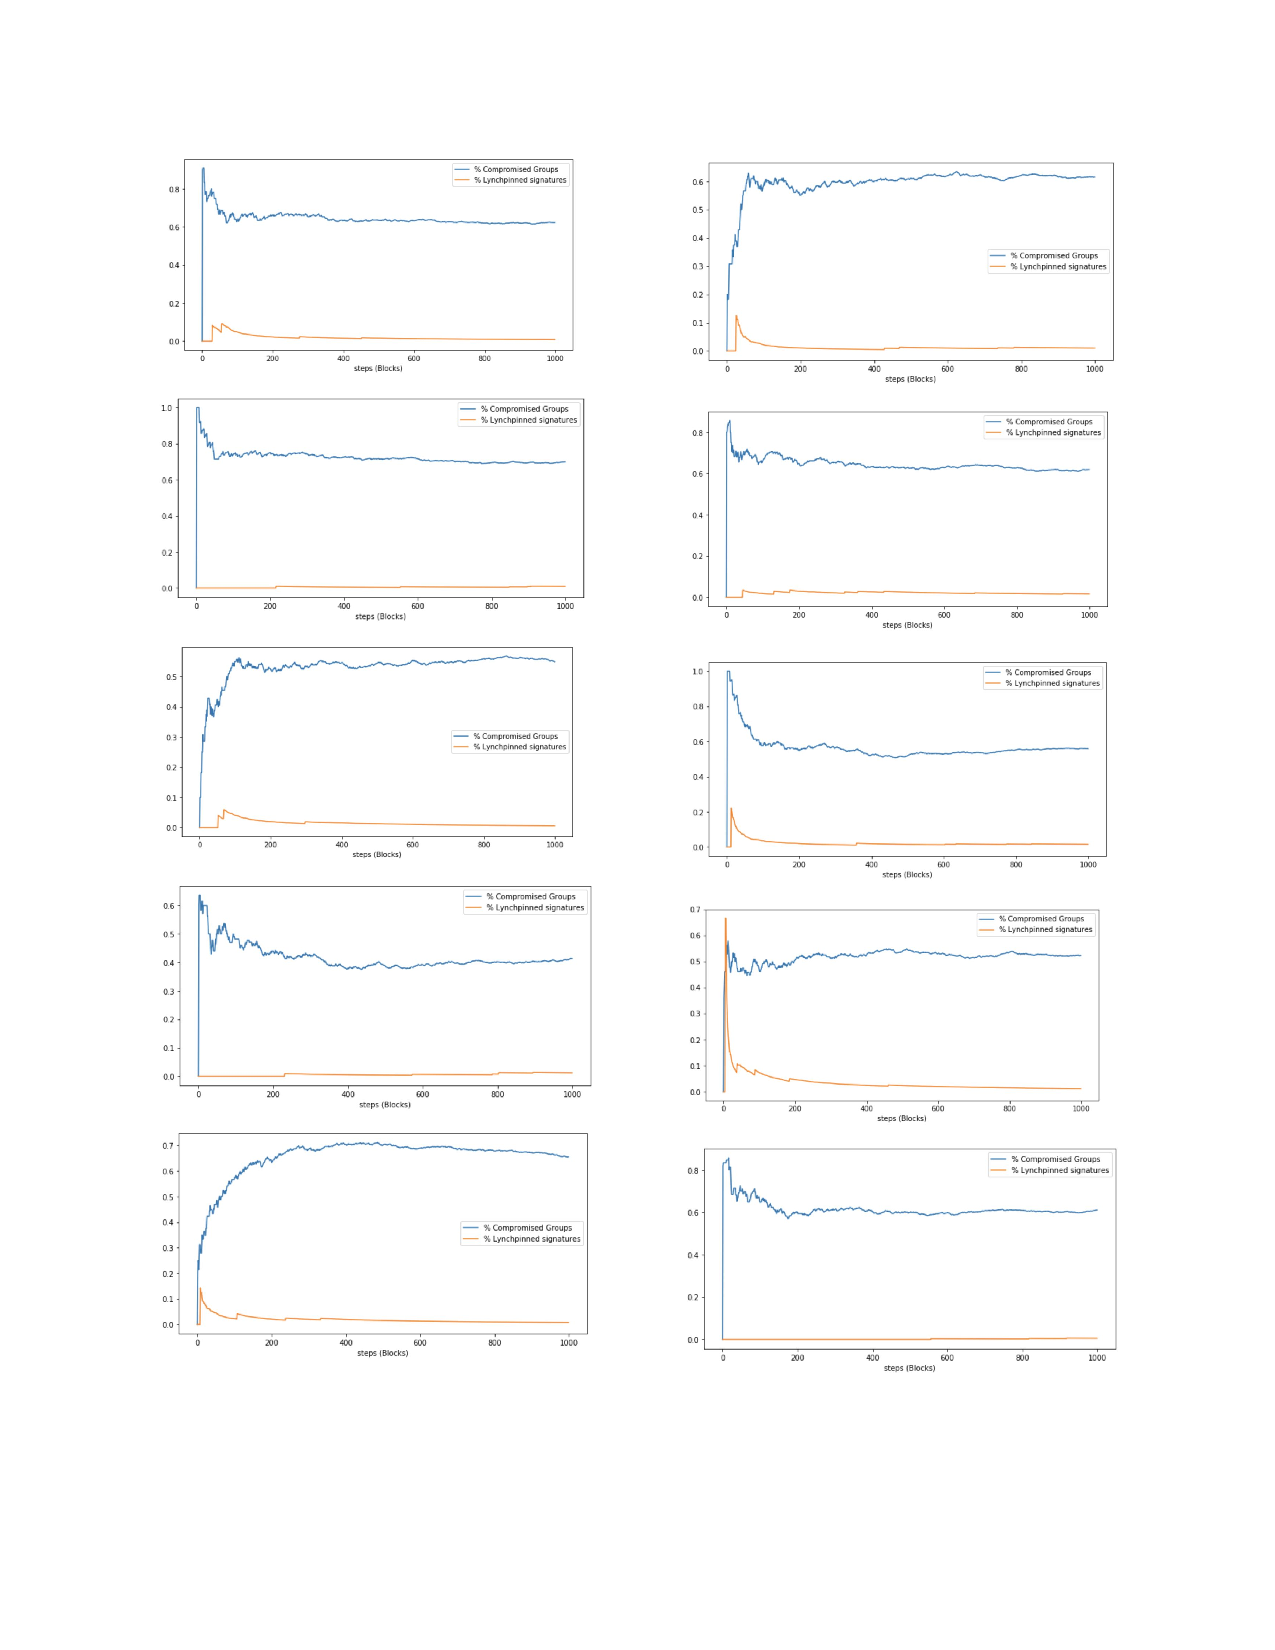
\includegraphics[width=\linewidth]{steady_state_behavior.pdf}
    \caption{Emergence of Steady State Behavior}
    \label{fig:steady_state}
\end{figure*}

\newpage
\begin{table}[htbp]
    \caption{Node Agent}
    \begin{center}
    \begin{tabular}{|c|c|}
    \cline{1-2} 
    \textbf{Key Attributes}&{\textbf{Node Agent}} \\
    \cline{1-2} 
    \hline
    Connection Delay & Delay between when a node is created and when it can join the network \\
    Ticket List & List of random numbers used to pick the node for participation in a group\\
    Connection Failure Percent & Likelihood of disconnecting from the network\\
    Death Percent & Likelihood of going offline and never re-connecting\\
    Malicousness & determines if a node is considered malicous based on if the operator is malicious\\
    Operator  & the entity that runs this node\\
    \hline
    \textbf{ }&\textbf{Group Agent} \\
    \hline
    Members & list of nodes that are members of the group. Nodes can repeat \\
    Expiry & number of blocks before group expires\\
    Malicious Percent & percentage of the groups members that are malicious\\
    Offline Percent & percentage of the groups members that are offline\\
    DKG Delay & User set delay simulating the distributed key generation process during group creation\\
    \hline
    \textbf{ }&\textbf{Signature Agent} \\
    \hline
    Group & list of nodes that are members of the group. Nodes can repeat \\
    Expiry & number of blocks before group expires\\
    Delay &  user specified time between being triggered and being published on chain\\
    Offline Percent & percentage of the groups members that are offline at the time of the signature\\
    Lynchpin operator percent & percent of the group owned by a single operator\\
    \hline
    \multicolumn{2}{l}{$^{\mathrm{a}}$Sample of a Table footnote.}
    \end{tabular}
    \label{agent_table}
    \end{center}
    \end{table}

\end{document}
